\section{배경 지식}

\subsection*{복소수의 극형식과 복소평면}

\begin{frame}
    \frametitle{복소수}
    \textit{잠시 고등학교로 돌아가서...} \pause
    \begin{itemize}
        \item \textbf{복소수}: \(z = a + bi \in \C\), (\(a, b \in \R\)) \pause
        \item 복소수의 덧셈/뺄셈
              \[
                  (a + bi) \pm (c + di) = (a \pm c) + (b \pm d)i
              \] \pause
        \item 복소수의 곱셈
              \[
                  (a + bi)(c + di) = (ac - bd) + (bc + ad)i
              \] \pause
        \item 복소수의 나눗셈
              \[
                  \frac{a + bi}{c + di} = \frac{a + bi}{c + di} \cdot \frac{c - di}{c - di} = \frac{(ac + bd) + (bc-ad)}{c^2 + d^2}
              \]
    \end{itemize}
\end{frame}

\begin{frame}
    \frametitle{복소평면}
    \begin{center}
        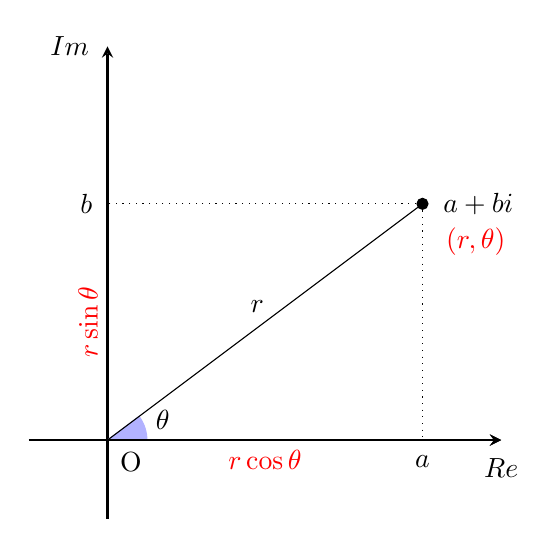
\begin{tikzpicture}
            \pgfmathsetmacro{\axislimit}{5}

            \node[below right=1pt] (origin) at (0,0) {\(\rm{O}\)};
            \draw [-stealth,thick] (-1, 0) -- (\axislimit, 0) node[below=3pt] {\(\mf{Re}\)};
            \draw [-stealth,thick] (0, -1) -- (0, \axislimit) node[left=3pt] {\(\mf{Im}\)};

            \onslide<2->{
                \coordinate (point) at (4, 3);
                \filldraw[fill=black] (point) circle (0.07);
                \node [right=4pt] at (point) {\(a + bi\)};
                \draw [dotted] (point) -- (4, 0);
                \draw [dotted] (point) -- (0, 3);

                \node [below=2pt] at (4, 0) {\(a\)};
                \node [left=2pt] at (0, 3) {\(b\)};
            }

            \onslide<3-> {
                \filldraw[color=blue!30] (0.5, 0) arc (0:36.869:0.5) -- (0, 0);
                \draw (0, 0) -- (point);
                \draw [-stealth,thick] (-1, 0) -- (\axislimit, 0);
                \node at (0.7, 0.25) {\(\theta\)};
                \node at (1.9, 1.7) {\(r\)};
            }

            \onslide<4-> {
                \node [below right=5pt, color=red] at (point) {\((r, \theta)\)};
                \node [below, color=red] at (2, 0) {\(r\cos\theta\)};
                \node [above, color=red, rotate=90] at (0, 1.5) {\(r\sin\theta\)};
            }
        \end{tikzpicture}
    \end{center}
\end{frame}


\begin{frame}
    \frametitle{복소수의 극형식}
    \begin{itemize}
        \item \alert{극형식}(polar form): \(z = (r, \theta) = r(\cos\theta + i\sin\theta)\) \pause
              \medskip
              \begin{itemize}
                  \item \(r = \abs{z} = \sqrt{a^2 + b^2}\) (원점과의 거리)
                        \medskip
                  \item \(\theta = \arg{z}\) (실수 축의 양의 방향과 이루는 각) \pause
              \end{itemize}
              \medskip
        \item 곱셈
              \[
                  (r_1, \theta_1) \cdot (r_2, \theta_2) = (r_1 r_2, \theta_1 + \theta_2)
              \]
        \item 나눗셈
              \[
                  \frac{(r_1, \theta_1)}{(r_2, \theta_2)} = \left(\frac{r_1}{r_2}, \theta_1 - \theta_2\right)
              \] \pause
        \item 손쉬워진 곱셈과 나눗셈!
    \end{itemize}
\end{frame}

\subsection*{Roots of Unity}
\begin{frame}
    \frametitle{Roots of Unity}
    \begin{theorem}[드 무아브르의 정리]
        복소수 \(z = (r, \theta)\)\,에 대하여,
        \begin{center}
            \(z^n = (r, \theta)^n = (r^n, n\theta)\)
        \end{center}
    \end{theorem}

    \pause

    \begin{itemize}
        \item \(n\)\,제곱 하면 거리는 \(n\)\,제곱 되고 각은 \(n\)\,배가 된다. \pause
        \item \alert{방정식 \(z^n = 1\) 의 해는?}
    \end{itemize}
\end{frame}

\begin{frame}
    \frametitle{Roots of Unity}
    \begin{itemize}
        \setlength{\itemsep}{1em}
        \item \(z = (r, \theta)\)\,라고 하면, \(z^n = (r^n, n\theta)\). \pause
        \item \(1 = (1, 2k\pi)\)\,이므로 (\(k\): 정수)
              \vspace*{10px}
              \begin{center}
                  \(r^n = 1\) and \(n\theta = 2k\pi\)
              \end{center} \pause
        \item \(r \geq 0\)\,이고 \(z^n = 1\)\,은 정확히 \(n\)\,개의 해를 가지므로,
              \vspace*{10px}
              \begin{center}
                  \alert{\(r = 1\)} and \alert{\(\ds \theta = \frac{2k\pi}{n}\)} \quad \((k = 0, \dots, n - 1)\)
              \end{center} \pause
        \item 이 \(n\)\,개의 해를 \alert{roots of unity}\,라 하고 \(\ds \omega_n = \left(1, \frac{2\pi}{n}\right)\)\,으로 표기
    \end{itemize}
\end{frame}

\begin{frame}
    \frametitle{예: \(z^7 = 1\) 의 해}
    \begin{center}
        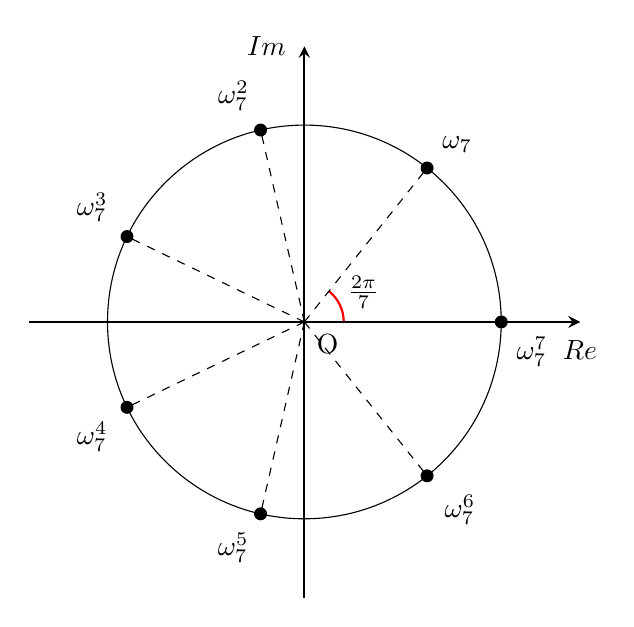
\begin{tikzpicture}[scale=2.5]
            \pgfmathsetmacro{\axislimit}{1.4}

            \node[below right=1pt] (origin) at (0,0) {\(\rm{O}\)};
            \draw [-stealth,thick] (-\axislimit, 0) -- (\axislimit, 0) node[below=3pt] {\(\mf{Re}\)};
            \draw [-stealth,thick] (0, -\axislimit) -- (0, \axislimit) node[left=3pt] {\(\mf{Im}\)};

            \coordinate (one) at (1, 0);
            \filldraw[fill=black] (one) circle (0.03) node[below right=2pt] {\(1\)};

            \onslide<2->{
                \coordinate (omega1) at (360/7:1);
                \filldraw[fill=black] (omega1) circle (0.03) node[above right=2pt] {\(\omega_7\)};
                \draw[color=red,thick] (0.2, 0) arc (0:360/7:0.2);
                \node at (0.3, 0.15) {\(\frac{2\pi}{7}\)};
                \draw[dashed] (0, 0) -- (omega1);
                \draw [-stealth,thick] (-\axislimit, 0) -- (\axislimit, 0);
            }

            \onslide<3-> {
                \draw (0, 0) circle (1);
            }

            \onslide<4->{
                \foreach \k in {2, 3, 4, 5, 6} {
                        \filldraw[fill=black] (360/7 * \k:1) circle (0.03);
                        \node[label=360/7 * \k:\(\omega_7^{\k}\)] at (360/7 * \k:1) {};
                        \draw[dashed] (0, 0) -- (360/7 * \k:1);
                    }

                \node[below right=2pt, fill=white] at (1, 0) {\(\omega_7^7\)};
            }
        \end{tikzpicture}
    \end{center}
\end{frame}

\begin{frame}
    \frametitle{\(\omega_n\) 의 성질}

    % n제곱 해야 1, 그 전엔 절대 1 아님
    % 또 FFT 증명에 사용되는 성질 하나 넣기

    \begin{columns}
        \column{0.5\textwidth}
        \begin{itemize}
            \item \(\omega_n^k \neq 1\) for \(1 \leq k \leq n - 1\)
                  \medskip
            \item \alert{\(\omega_n^n = 1\)}
                  \medskip
            \item<2->{짝수 \(n\)에 대하여,
                  \medskip
                  \begin{itemize}
                      \item \alert{\(\omega_n^{n/2} = -1\)}
                            \medskip
                      \item \(\omega_n^{\alert{2}} = \omega_{n/\alert{2}}\)
                  \end{itemize}}
        \end{itemize}

        \column{0.55\textwidth}
        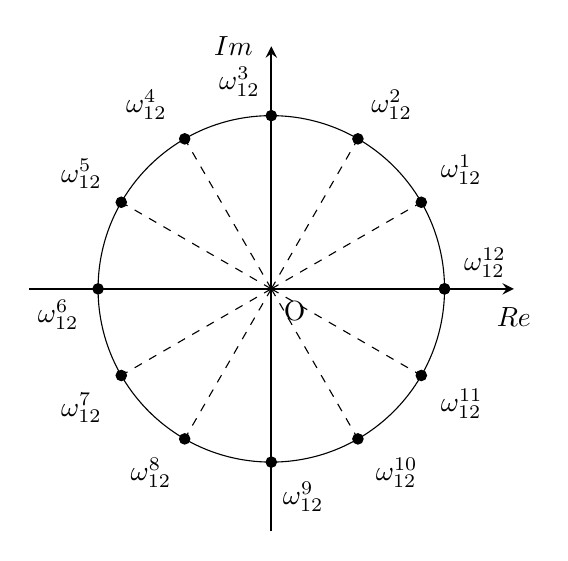
\begin{tikzpicture}[scale=2.2]
            \pgfmathsetmacro{\axislimit}{1.4}
            \pgfmathsetmacro{\n}{12}
            \node[below right=1pt] (origin) at (0,0) {\(\rm{O}\)};
            \draw [-stealth,thick] (-\axislimit, 0) -- (\axislimit, 0) node[below=3pt] {\(\mf{Re}\)};
            \draw [-stealth,thick] (0, -\axislimit) -- (0, \axislimit) node[left=3pt] {\(\mf{Im}\)};

            \coordinate (one) at (1, 0);
            \filldraw[fill=black] (one) circle (0.03);
            \draw (0, 0) circle (1);

            \foreach \k in {1, ..., \n} {
                    \filldraw[fill=black] (360/\n * \k:1) circle (0.03);
                    \node[label=360/\n * \k + 10:\(\omega_{\n}^{\k}\)] at (360/\n * \k:1) {};
                    \draw[dashed] (0, 0) -- (360/\n * \k:1);
                }
        \end{tikzpicture}
    \end{columns}
\end{frame}

\begin{frame}
    \begin{center}

        \begin{tikzpicture}[scale=2.5]
            \pgfmathsetmacro{\axislimit}{1.4}
            \pgfmathsetmacro{\n}{12}
            \node[color=white,label={30:\(\color{white} {\omega_{6}^6} = \omega_{12}^{12}\)}] at (360:1) {};
            \node[below right=1pt] (origin) at (0,0) {\(\rm{O}\)};
            \draw [-stealth,thick] (-\axislimit, 0) -- (\axislimit, 0) node[below=3pt] {\(\mf{Re}\)};
            \draw [-stealth,thick] (0, -\axislimit) -- (0, \axislimit) node[left=3pt] {\(\mf{Im}\)};
            \coordinate (one) at (1, 0);
            \draw (0, 0) circle (1);

            \only<1> {
                \filldraw[fill=black] (one) circle (0.03);
                \foreach \k in {1, ..., \n} {
                        \filldraw[fill=black] (360/\n * \k:1) circle (0.03);
                        \node[label=360/\n * \k + 10:\(\omega_{\n}^{\k}\)] at (360/\n * \k:1) {};
                        \draw[dashed] (0, 0) -- (360/\n * \k:1);
                    }
            }

            \only<2-> {
                \foreach \k in {1, ..., \n} {
                        \filldraw[fill=black] (360/\n * \k:1) circle (0.03);
                    }
                \draw[-stealth,thick,color=red] (35:1.15) arc (35:55:1.15);
                \node[label=0:\(\omega_{\n}\)] at (360/\n:1) {};

                \draw[-stealth,thick,color=red] (95:1.15) arc (95:175:1.15);
                \node[label=45:\(\omega_{\n}^3\)] at (360/\n * 3:1) {};

                \draw[-stealth,thick,color=red] (185:1.15) arc (185:355:1.15);
                \node[label=-45:\(\omega_{\n}^6\)] at (360/\n * 6:1) {};
            }

            \only<3> {
                \foreach \k in {1, ..., 6} {
                        \filldraw[fill=red] (60 * \k:1) circle (0.03);
                        \draw[color=red,dashed] (0, 0) -- (60 * \k:1);
                    }

                \node[color=red,label={80:\({\color{red}\omega_{6}} = \omega_{12}^2\)}] at (60:1) {};
                \node[color=red,label={30:\({\color{red}\omega_{6}^3} = \omega_{12}^6\)}] at (180:1) {};
                \node[color=red,label={30:\({\color{red}\omega_{6}^6} = \omega_{12}^{12}\)}] at (360:1) {};
            }
        \end{tikzpicture}
    \end{center}
\end{frame}

\subsection*{다항식}

\begin{frame}
    \frametitle{다항식}
    \begin{itemize}
        \setlength{\itemsep}{1em}
        \item \(R[x]\): Ring \(R\)\,의 원소를 계수로 갖는 다항식의 집합
              \smallskip
              \begin{itemize}
                  \item \(\R[x]\): 실수 계수 다항식의 집합
                        \smallskip
                  \item \(\Z_n[x]\): 정수 계수 다항식의 집합 (단, 계수는 모두 \(\rm{mod} \; n\))
              \end{itemize}

        \item<2-> 벡터로도 표기\footnote<2->{어차피 \(x\)는 symbol일 뿐...}
              \smallskip
              \begin{itemize}
                  \item \(f(x) = \ds \sum_{i=0}^{n-1} a_{i}x^i = a_0 + a_1x + a_2x^2 + \cdots + a_{n-1}x^{n-1}\)
                        \smallskip
                  \item \(f = \left(a_0, a_1, \dots, a_{n-1}\right)\)
              \end{itemize}

        \item<3-> 다항식 \(f(x)\)\,의 차수를 \(\deg f\)\,로 나타냄
        \item<4-> \(\Z_{10001}\)\,에서 \(x^2 - 1 = (x - 2191)(x - 7810)\) (!)
    \end{itemize}
\end{frame}

\subsection*{합동식}

\begin{frame}
    \frametitle{합동식}
    \begin{itemize}
        \setlength{\itemsep}{2em}
        \item 정수 \(a\)를 정수 \(b\)로 나눈 몫과 나머지가 각각 \(q,\,r\)일 때,
              \smallskip
              \begin{center}
                  \(a = bq + r\) \quad and \quad \(a \equiv r \pmod{b}\)
              \end{center}
              \smallskip
              \begin{itemize}
                  \item 프로그래밍 언어들에 존재하는 \textsc{\%} 연산
                        \medskip
                  \item \(17 \equiv 4 \pmod{13}\)
              \end{itemize}
        \item<2-> 다항식 \(A\)를 다항식 \(B\)로 나눈 몫과 나머지가 각각 \(Q,\,R\)일 때,
              \smallskip
              \begin{center}
                  \(A = BQ + R\) \quad and \quad \(A \equiv R \pmod{B}\)
              \end{center}
              \smallskip
              \begin{itemize}
                  \item<3-> \(x^2 + 5x + 4 = (x + 2)^2 + x\)
                        \medskip
                  \item<3-> \(x^2 + 5x + 4 \equiv x \pmod{(x + 2)^2}\)
              \end{itemize}
    \end{itemize}
\end{frame}
